\documentclass[10pt,english,a4paper]{article}

\usepackage[english]{babel}
\usepackage[IL2]{fontenc} 
\usepackage[utf8]{inputenc}
\usepackage{graphicx}
\usepackage{url} 
\usepackage{hyperref} 
\usepackage {lipsum}
\usepackage{cite}
\usepackage{subfig}
\usepackage{wrapfig}
\usepackage{amsmath}


\pagestyle{headings}

\title{Comparison of Blockchain usage in different sectors\centering\thanks{Semestral project in subject Methods of Engineering work, ac. the year 2023/2024}} 

\author{Zdenko Kanoš\\[2pt]
	{\small Slovak University of Technology in Bratislava}\\
	{\small Faculty of Informatics and Information Technologies}\\
	{\small \texttt{xkanos@stuba.sk}}
	}

\date{\small 28.09.2023} 



\begin{document}

\maketitle

\begin{abstract}
I was inspired to write this article by the article by Jarot Sembodo Suroso\cite{Suroso:SKCK} In my perspective, Blockchain represents the future of secure data storage, particularly for classified documents. The primary aim of my article is to emphasize Blockchain’s current and future utility. I was inspired by enlightening articles highlighting Blockchain's practical application in various real-world scenarios. Starting with an explanation of what Blockchain is and its evolution, these articles have paved my way to focus on sectors like police records, decentralized voting, or how government data can be stored on the Blockchain. In my article, I will also talk about why storing data on the Blockchain is better and more secure and what is different about the application of Blockchain in different sectors.
\end{abstract}

\section{Introduction}
Nowadays, in an era of unstoppable development, several technologies are still being developed. Such technologies enrich the quality of our lives and often bring us easier solutions to everyday problems and societal challenges. One of the problems of the society is that our data and information are not always secured enough and data breaches may occur during some hacker attacks. This can be very dangerous already for the ordinary user but even more dangerous for huge public institutions processing huge amounts of data. Another problem in terms of data security is that it is relatively easy to alter and falsify data.  This is where the Blockchain comes in, which makes all the data more secure, impossible to falsify and, if we want, more transparent, for example, in the process of electronic elections.
\newpage
\subsection{What is blockchain?}
\begin{wrapfigure}{l}{0.4\textwidth}
  \centering
  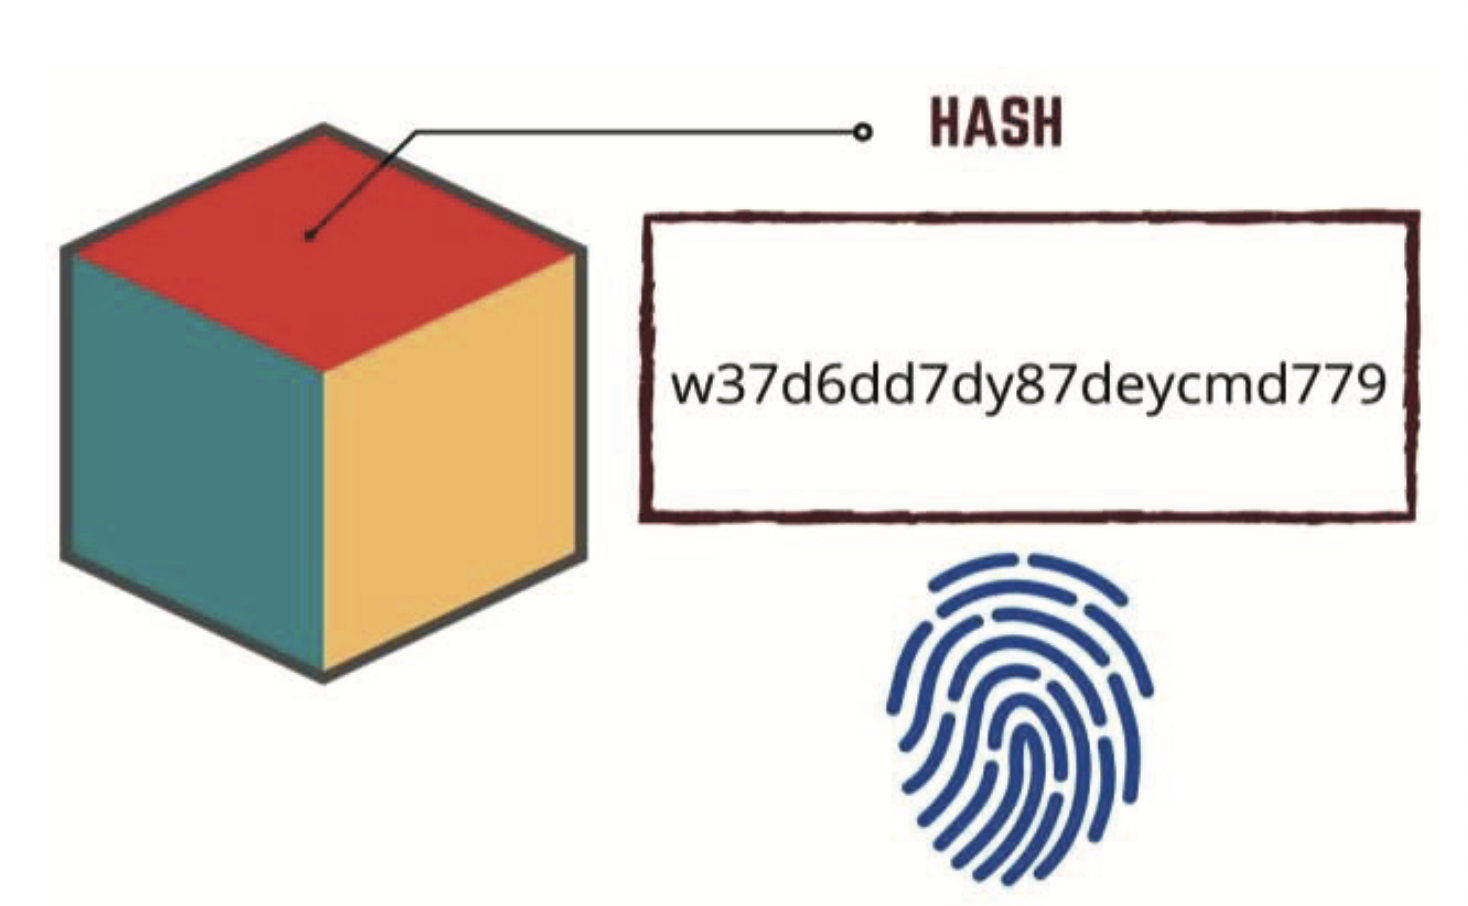
\includegraphics[width=0.37\textwidth]{Blockchain-hash.png} 
  \caption{Blockchain Hash\cite{Jain:Criminal:record}}
\end{wrapfigure} 
Blockchain according to Jarot Sembodo Suroso\cite{Suroso:SKCK} is a decentralized computer software featuring a database that acts as a global ledger, accessible across a network of Bitcoin users who operate on a peer-to-peer basis, adhering to a predefined protocol. Peer- to-peer connects from one computer to another in a large network of all Bitcoin users. To connect to Blockchain a cryptographic identity is required to access it, an email and a password. After a transaction the data cannot be changed because the data is assigned to a block. If someone wants to make adjustments for anything on the Blockchain, they would have to change every block on the Blockchain, this is  the reason why this is impossible. Because all of the network users would have to agree. Blockchain also records a chronological history of all transactions which have occurred in a series of block connected to each other.{Suroso:SKCK}

\subsection{Evolution path of Blockchain}
\begin{figure}[h]
    \centering
    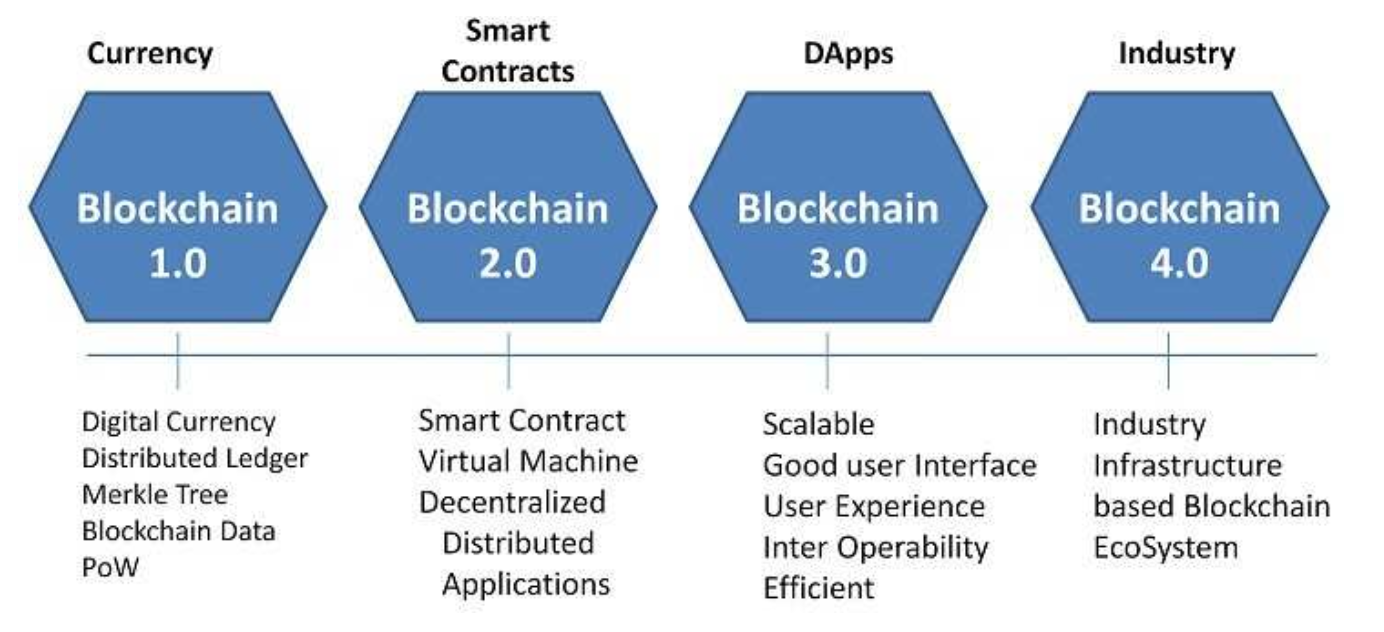
\includegraphics[scale=0.4]{Blockchain-evolution.png}
    \caption{Blockchain Evolution Path \cite{Suroso:SKCK}}
    \label{histogram}
\end{figure}
\paragraph{Blockchain 1.O}
This period marked the emergence of Distributed Ledger Technology (DLT) being applied to create its initial cryptocurrency application, Bitcoin, which enables digital payments.
\cite{Suroso:SKCK}
\paragraph{Blockchain 2.O}
The Smart Contract feature was introduced as a solution to address the limitations of Blockchain 1.0. Smart Contracts are essentially automated computer programs that execute based on predefined conditions.
\cite{Suroso:SKCK}
\paragraph{Blockchain 3.0}
During this era, DApps were introduced, representing blockchain-based applications with decentralized storage and communication capabilities. These applications primarily operate with backend code on decentralized networks, in contrast to conventional applications that rely on centralized servers.
\cite{Suroso:SKCK}
\paragraph{Blockchain 4.0}
Leveraging the capabilities of Blockchain 3.0 to address the requirements of Industry 4.0. Industry 4.0 focuses on trust, privacy, automation, and seamless system integration. Thanks to its decentralized architecture, it can effectively withstand malicious attacks and fraud.
\cite{Suroso:SKCK}

\subsection{Blockchain security}
As i mentioned in the evolution of Blockchain. The main beauty of a Blockchain is it's security. Which is thanks to the three main key elements mentioned in the last section:

\begin{itemize}
    \item Distributed ledger technology:
    \item Immutable records:
    \item Smart Contracts:
\end{itemize}
   
  

\section{Blockchain based criminal record database}

Blockchain is technology which is common in Industry 4.0. However, not many governments have implemented it yet into the government segment. Even though it is a very important thing to create a safe and transparent system. \cite{Suroso:SKCK}(clanok2)Criminal records are crucial in the interrogation and detection of a crime. Even high level governments have problems managing and using these data. \cite{Jain:Criminal:record}(clanok1)  So that is why they researched a system for making Police Record Certificates in SKCK (Surat Keterangan Catatan Kepolisian) in Indonesia.  The conclusion of this research is that Blockchain implementation is very necessary because it can make data and information more secure and verifiable using hashes. \cite{Suroso:SKCK}(clanok2)
\\
Blockchain promises transparent tamper-proof, and secure systems. Many institutions, and also international governments have interest in Blockchain technology but they did not implement the Blockchain into the government yet.\cite{Suroso:SKCK} 
		

  \begin{figure}[h]
  \centering
   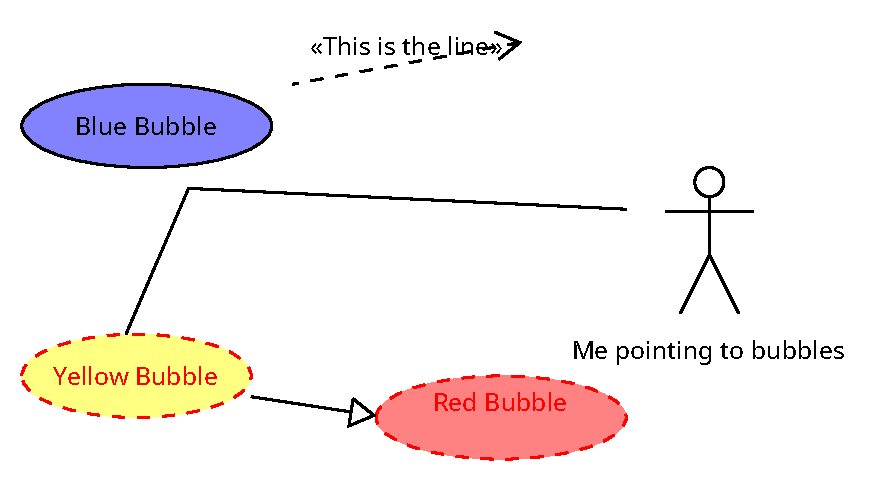
\includegraphics[scale=0.8]{Diagram_1.pdf}
  \centering
  \caption{Diagram}
 \end{figure}
 \lipsum[1-2]
 
 \begin{figure}%
    \centering
    \subfloat[\centering label 1]{{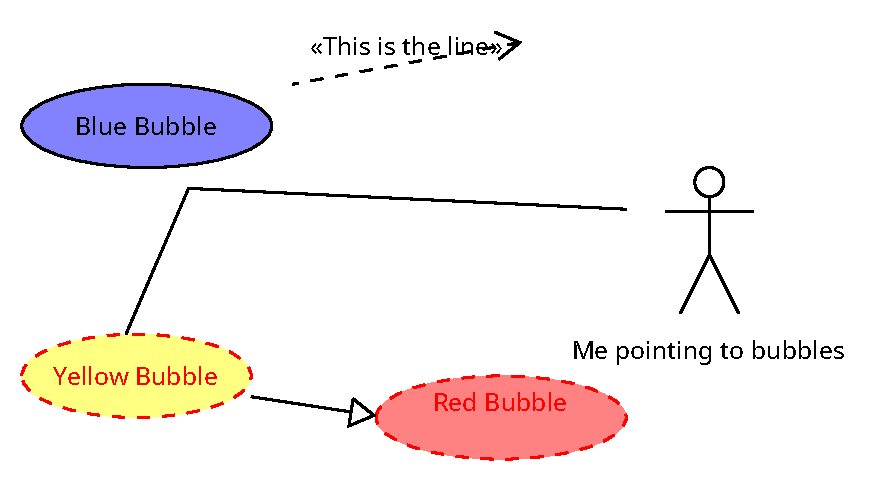
\includegraphics[width=5cm]{Diagram_1.pdf} }}%
    \qquad
    \subfloat[\centering label 2]{{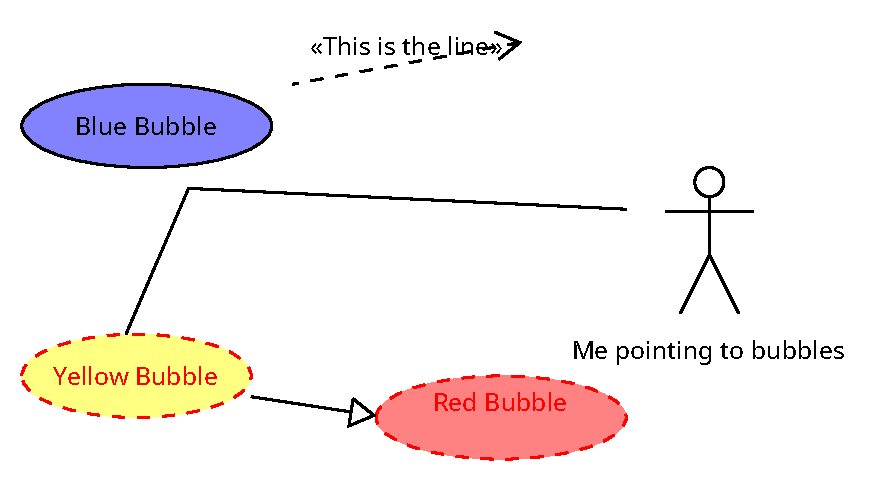
\includegraphics[width=5cm]{Diagram_1.pdf} }}%
    \caption{2 Figures side by side}%
    \label{fig:example}%
\end{figure}
 
 \lipsum[1-3]

 \section{Sekcia 2}
 \lipsum[1-2]
 \begin{wrapfigure}{r}{0.5\textwidth}
  \centering
  
\includegraphics[width=0.48\textwidth]{STU-FIIT-ancv.png} 
  \caption{Test Diagram}
\end{wrapfigure} 
 \lipsum[1-4]
 
$\begin{bmatrix}
  a & b & c & d & e &f\\
  g & h & i & j & k &l \\
  m & n & o & p & r &s\\
   a & b & c & d & e &f\\
  g & h & i & j & k &l \\
  m & n & o & p & r &s\\
  

  
\end{bmatrix}$



 
\bibliography{literatura}
\bibliographystyle{abbrv}
\end{document}
